%%%%%%%%%%%%%%%%%%%%%%%%%%%%%%%%%%%%%%%%%
% University/School Laboratory Report
% LaTeX Template
% Version 3.1 (25/3/14)
%
% This template has been downloaded from:
% http://www.LaTeXTemplates.com
%
% Original author:
% Linux and Unix Users Group at Virginia Tech Wiki 
% (https://vtluug.org/wiki/Example_LaTeX_chem_lab_report)
%
% License:
% CC BY-NC-SA 3.0 (http://creativecommons.org/licenses/by-nc-sa/3.0/)
%
%%%%%%%%%%%%%%%%%%%%%%%%%%%%%%%%%%%%%%%%%

%----------------------------------------------------------------------------------------
%	PACKAGES AND DOCUMENT CONFIGURATIONS
%----------------------------------------------------------------------------------------

\documentclass{article}

\usepackage[version=3]{mhchem} % Package for chemical equation typesetting
\usepackage{siunitx} % Provides the \SI{}{} and \si{} command for typesetting SI units
\usepackage{graphicx} % Required for the inclusion of images
\usepackage{natbib} % Required to change bibliography style to APA
\usepackage{amsmath} % Required for some math elements 
\usepackage{caption}
\usepackage{subcaption}

\setlength\parindent{0pt} % Removes all indentation from paragraphs

\renewcommand{\labelenumi}{\alph{enumi}.} % Make numbering in the enumerate environment by letter rather than number (e.g. section 6)

\newcommand\tab[1][0.5cm]{\hspace*{#1}}

%\usepackage{times} % Uncomment to use the Times New Roman font

%----------------------------------------------------------------------------------------
%	DOCUMENT INFORMATION
%----------------------------------------------------------------------------------------

\title{COMP 429/529: Project 1} % Title

\author{Berkay \textsc{Barlas}} % Author name

\date{\today} % Date for the report

\begin{document}

\maketitle % Insert the title, author and date

\begin{center}
\begin{tabular}{l r}
Date Performed: & March 17, 2019 \\ % Date the experiment was performed
Instructor: & Didem Unat % Instructor/supervisor
\end{tabular}
\end{center}

% If you wish to include an abstract, uncomment the lines below
% \begin{abstract}
% Abstract text
% \end{abstract}

%----------------------------------------------------------------------------------------
%	SECTION 1
%----------------------------------------------------------------------------------------

In this assignment I developed my parallel implementations 
on top of given serial version for two different applications;
\newline an image blurring algorithm and sudoku solver using OpenMP. 
\newline While the first application in data parallelism, 
the second application in task parallelism. 
\newline
\newline
In this assignment I have completed
\begin{itemize}
    \item Parallel Version of Image Blurring
    \item Performance Study for Part I
    \item Parallel Version of Sudoku Part A, Part B, Part C
    \item Performance Study for Part II 
\end{itemize}


\section{Part I: Image Blurring}


\tab{} In the first part of this assignment I implemented a parallel version of a simple image blurring algorithm with OpenMP which takes an input image and outputs a blurred image.
\\
\tab{} The image is represented as a 2-dimensional grid with three components.  
After reading the image to be filtered, the program generates an n by n filter. 
The filter is then applied to blur every pixel in the image. 
For pixels which are located along/near the edges of the image, zero padding technique is used to add additional zero-valued pixels beyond the edges of the image.

%\begin{center}\ce{2 Mg + O2 -> 2 MgO}\end{center}

\newpage
\subsection{Stability Test}

\begin{description}
    \item[Serial version execution time: ] \hfill \\ 
    Coffee Image: 13.64\\
    Strawberry Image: 27.56\\
    \item[Paralel version with single thread execution time: ] \hfill \\
    Coffee Image: 30.88\\
    Strawberry Image: 55.93\\
    \item[Which thread number gives best performance?] \hfill \\
    32 thread count gives best performance for both blurring applications.
    \\
    The reason of serial version performs better than parallel version with 1 thread is Parallization overhead.
    The difference between them caused by the execution time of parallization.
\end{description}

\textbf{Results}

\begin{figure}[!htb]
    \centering
    \begin{subfigure}{.45\textwidth}
        \centering
        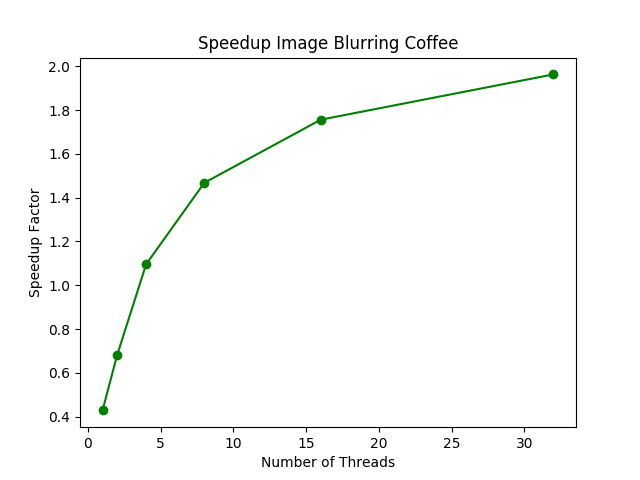
\includegraphics[width=1\linewidth]{./img/speedup_part_1_A.png}
        \caption{Speedup results for the blurring on coffee image.}
    \end{subfigure} 
    \begin{subfigure}{.45\textwidth}
        \centering
        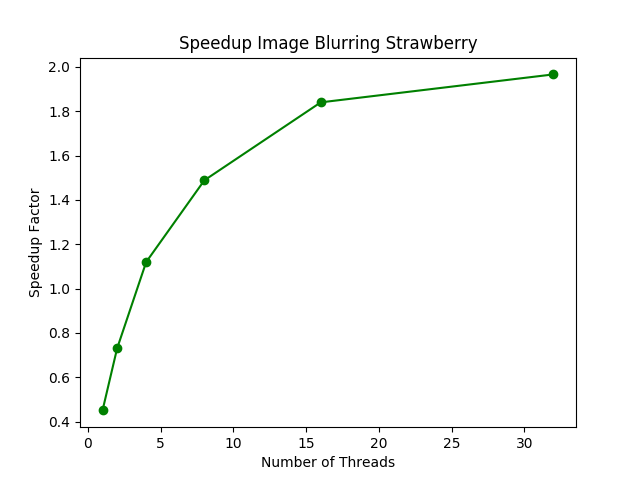
\includegraphics[width=1\linewidth]{./img/speedup_part_1_A_strawberry.png}
        \caption{Speedup results for the blurring on strawberry image.}
    \end{subfigure}
    \caption{Speedup figures for image blurring application}
\end{figure}   

\textbf{Explanation of Speedup Curve}
\\
\tab Even though, a linear/perfect speedup is not expected the results are actually worse than what is expected.\\
The reasons of that is some part of the code is non-parallelizable such as ...\\
The 32 thread parallel version on 32 core cluster gives only around 2x speedup.\\

\newpage

\subsection{Thread Binding Test}
\tab In the compact mapping, multiple threads are mapped as close as possible to each other, 
while in the scatter mapping, the threads are distributed as evenly as possible across all cores. 

\begin{description}
    \item[Different mapping strategies; Compact and Scatter]
\end{description}
\textbf{Results}
 \begin{figure}[!htb]
    \centering
    \begin{subfigure}{.45\textwidth}
        \centering
        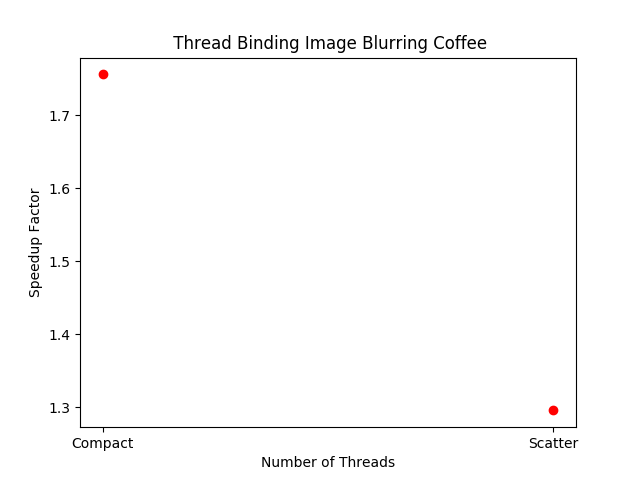
\includegraphics[width=1\linewidth]{./img/binding_part_1_B_coffee.png}
        \caption{Results for the blurring on coffee image.}
    \end{subfigure} 
    \begin{subfigure}{.45\textwidth}
        \centering
        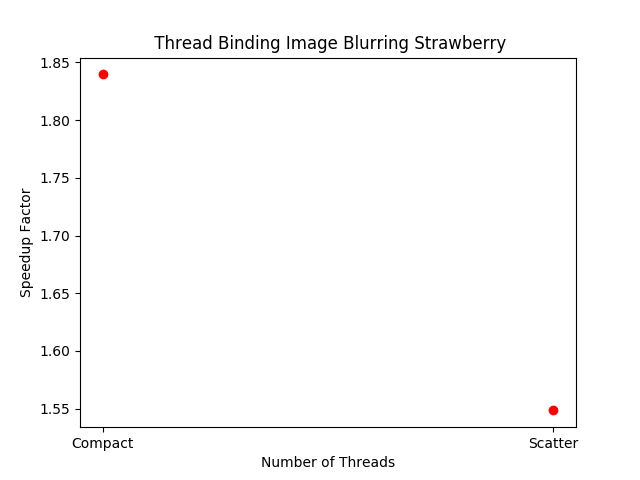
\includegraphics[width=1\linewidth]{./img/binding_part_1_B_strawberry.png}
        \caption{Results for the blurring on strawberry image.}
    \end{subfigure}
    \caption{Speedup figures for image blurring application}
\end{figure}

Which Mapping Gives Better Performance, Why?\\
\\ \tab Compact gives better performance for both images because 
when neighbouring threads are accessing the same or nearby data;
the data which is brought into the cache by one thread can be used 
by the other, avoiding a costly memory access.
\\ Talk about Caching.

%----------------------------------------------------------------------------------------
%	SECTION 2
%----------------------------------------------------------------------------------------
\newpage

\section{PART II: Parallel Sudoku Solver}
\tab In the second part of this assignment, I parallelized a serial sudoku solver with OpenMP
which takes a sudoku problem as an input and finds all possible solutions from it 
using a brute force search for searching by all possible solutions to the problem. 

\subsection{Scalability Test}
\subsubsection{Part A}
\begin{description}
\item[Serial version execution time: ] 48.10
\item[Paralel version with single thread execution time: ] 78.69
\item[Which thread number gives best performance?]\hfill \\
32 thread count gives best performance.
\end{description} 

\textbf{Results}
 \begin{figure}[!htb]
    \centering
        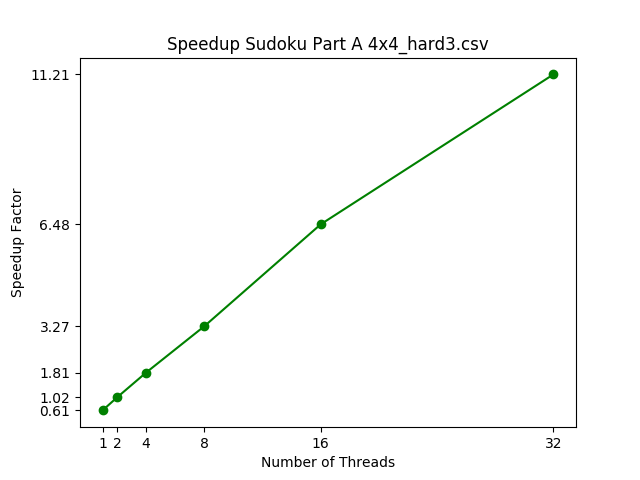
\includegraphics[width=0.8\linewidth]{./img/speedup_part_2_A.png}
        \caption{\small Results for the Sudoku 4x4hard3 using algorithm in.}
\end{figure}                

\textbf{Explanation of Speedup Curve}\\
\tab The task Parallization of serial version results in the creation of too many different task
which causes to a great overhead.
Therefore, the speedup results are lower than expected. Even with 32 thread speedup is just around 2.
\tab WHY IS NOT LINEAR
\newpage

\subsubsection{Part B}

\begin{description}
\item[Serial version execution time: ] 48.10
\item[Paralel version with single thread execution time: ] 74.50
\item[Which thread number gives best performance?]\hfill \\
32 thread count gives best performance.

\end{description} 
\begin{figure}[!htb]
        \centering
        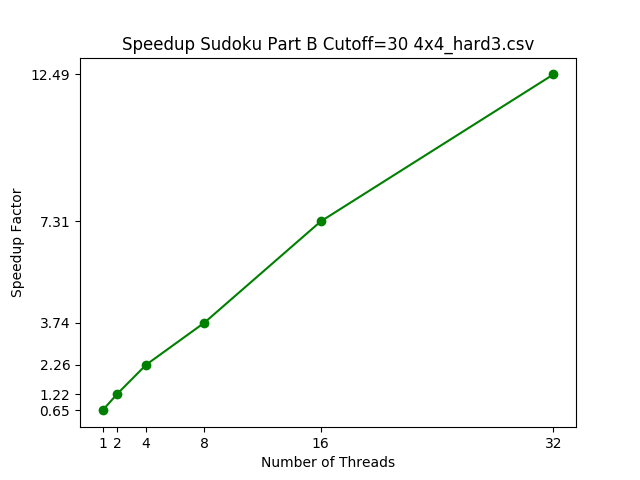
\includegraphics[width=1\linewidth]{./img/speedup_part_2_B.png}
        \caption{Results for the blurring on strawberry image.}
\end{figure}
\textbf{Explanation of Speedup Curve}\\
\tab In order to improve the performance of the previous parallel version, a cutoff parameter 
to limit the number of parallel tasks is needed.\\
\tab I defined a variable called depth and passed it as parameter to recursive method  
to prevent task creation after certain depth in the call-path tree. 
After that depth switch to the serial execution and do not generate more tasks.
To determine that cut off parameter, I executed parallel program with several
different values.\\
\tab The speedup curve is linear which is expected.  

\newpage

\subsubsection{Part C}
\tab Stopping the execution after finding a solution is very easy for 
serial version which can be done by returning a different value 
inside of for loops when a solution is found.
\newline
\tab In order to guraantee single solution in parallel version a shared variable 'found'
which will stop further task creation and execution can be defined.
\begin{description}
\item[Serial version execution time: ] 0.33
\item[Paralel version with single thread execution time: ] 0.57
\item[Which thread number gives best performance?]\hfill \\
32 thread count gives best performance.
\end{description} 

\begin{figure}[!htb]
        \centering
        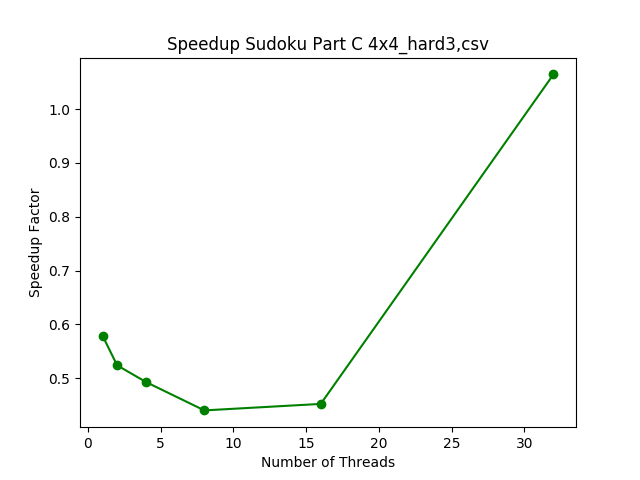
\includegraphics[width=1\linewidth]{./img/speedup_part_2_C.png}
        \caption{Results for the blurring on strawberry image.}
\end{figure}
\textbf{Explanation of Speedup Curve}
\\
\tab 
\newpage

\subsection{Thread Binding Test}
\subsubsection{Part A}
\begin{description}
    \item[Different mapping strategies; Compact and Scatter]
\end{description}
\begin{figure}[!htb]
    \centering
    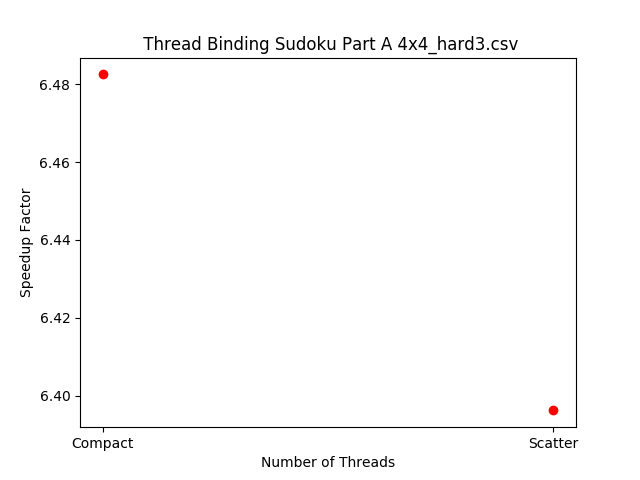
\includegraphics[width=1\linewidth]{./img/binding_part_2_A.png}
    \caption{Results for the blurring on strawberry image.}
\end{figure}
\textbf{Which Mapping Gives Better Performance, Why?}\\
\\ \tab Compact gives better performance for both images because 
when neighbouring threads are accessing the same or nearby data;
the data which is brought into the cache by one thread can be used 
by the other, avoiding a costly memory access.
\\ Talk about Caching.


\newpage

\subsubsection{Part B}
\begin{description}
    \item[Different mapping strategies; Compact and Scatter]
\end{description}
\begin{figure}[!htb]
    \centering
    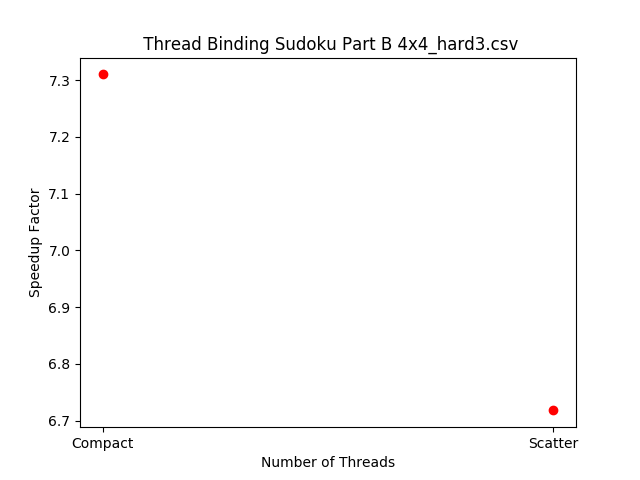
\includegraphics[width=1\linewidth]{./img/binding_part_2_B.png}
    \caption{Results for the blurring on strawberry image.}
\end{figure}
\textbf{Which Mapping Gives Better Performance, Why?}\\
\\ \tab Compact gives better performance for both images because 
when neighbouring threads are accessing the same or nearby data;
the data which is brought into the cache by one thread can be used 
by the other, avoiding a costly memory access.
\\ Talk about Caching.

\newpage

\subsubsection{Part C}
\begin{description}
    \item[Different mapping strategies; Compact and Scatter]
\end{description}
\begin{figure}[!htb]
    \centering
    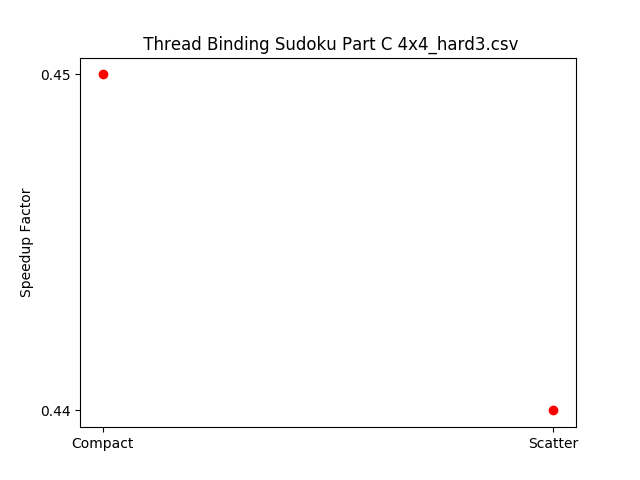
\includegraphics[width=1\linewidth]{./img/binding_part_2_C.png}
    \caption{Results for the blurring on strawberry image.}
\end{figure}
\textbf{Which Mapping Gives Better Performance, Why?}\\
\\ \tab Compact gives better performance for both images because 
when neighbouring threads are accessing the same or nearby data;
the data which is brought into the cache by one thread can be used 
by the other, avoiding a costly memory access.
\\ Talk about Caching.

\newpage

\subsection{Tests on Sudoku Problems of Different Grids}
\begin{description}
\item[Part-B]
\end{description} 
\begin{figure}[!htb]
    \centering
    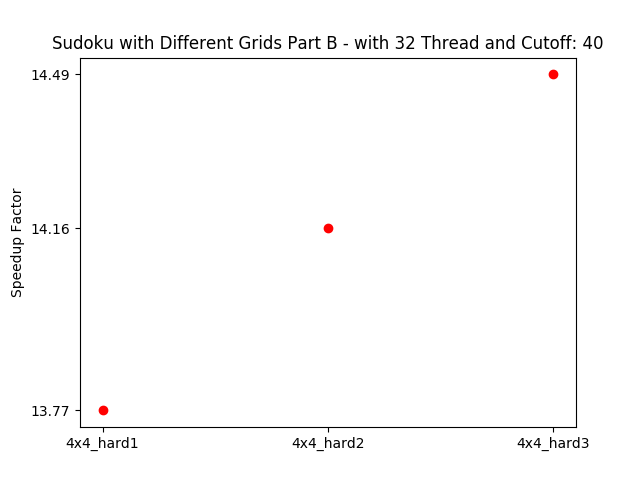
\includegraphics[width=1\linewidth]{./img/grids_part_2_B.png}
    \caption{Results for the 32 Thread Parallel Sudoku solver in Part B with different sizes and difficulties.}
\end{figure}


%----------------------------------------------------------------------------------------
%	SECTION 6
%----------------------------------------------------------------------------------------

\section{Formulas Used}

\begin{enumerate}
\begin{item}
\emph{Speedup} 
\begin{equation*}
\frac{\mathrm{T1}}{\mathrm{Tp}}
%\begin{center}\ce{}\end{center}
\end{equation*}
\begin{center}\ce{Speedup = T1 / Tp}\end{center}
\end{item}
\end{enumerate}




\end{document}